% Manuscript reconstructed from frozen experiment artifacts.
% Target journal: Fractal and Fractional, Section Optimization, Big Data, and AI/ML.
\documentclass[fractalfract,article,submit,moreauthors,pdftex]{Definitions/mdpi}

\firstpage{1}
\makeatletter
\setcounter{page}{\@firstpage}
\makeatother
\pubvolume{1}
\issuenum{1}
\articlenumber{0}
\pubyear{2026}
\copyrightyear{2026}
\datereceived{}
\dateaccepted{}
\datepublished{}
\setlength{\emergencystretch}{3em}
\setlength{\headheight}{20pt}

\Title{Endpoint-Constrained Multi-Band Fractional Memory for Repairing Long-Duration Limb Occlusions in Dance Motion Capture}
\Author{Lei Liu $^{1}$ and Zhantu Liang $^{2,*}$}
\AuthorNames{Lei Liu and Zhantu Liang}
\address{%
$^{1}$ \quad Physical Education Teaching and Research Section, Xi'an Innovation College of Yan'an University, Zaohe Road 2, Weiqu Subdistrict, Chang'an District, Xi'an 710100, Shaanxi, China; liu290031937@gmail.com\\
$^{2}$ \quad Institute of Ultrasonic Technology, Shenzhen Polytechnic University, Shenzhen 518055, China}
\corres{Correspondence: liangzhantu@szpu.edu.cn}

\abstract{Markerless dance capture can lose distal joints during fast self-occlusion, producing gaps that disrupt kinematic analysis. We present an endpoint-constrained multi-band fractional memory bridge for long localized gaps in 3D dance skeletons. Three truncated Grunwald--Letnikov fractional-integral kernels aggregate visible motion increments, and bidirectional context is converted into a correction that is analytically zero at both observed gap endpoints. We evaluated 1,408 AIST++ sequences using a choreography-grouped split, three training seeds, 221 held-out sequences, and a finite-window bridge matched in surrounding architecture and nominal parameters. A broad development hypothesis across missingness patterns was not supported; a focused 72-frame limb-occlusion hypothesis was then fixed before test access. The fractional system reduced mean per-joint position error relative to the finite bridge in every seed, with a paired sequence-bootstrap gain of 0.279\% (95\% confidence interval: 0.167--0.387\%). A post-confirmatory control trained without the fractional trajectory loss retained a 0.293\% gain (95\% confidence interval: 0.184--0.400\%), showing that the positional improvement persists without that auxiliary loss. An exploratory sweep found gains for localized gaps of 60--96 frames, whereas uniform full-body gaps favored finite memory. The 3.02M-parameter system processed a 128-frame window in 14.16 ms on an RTX 3090. The evidence supports fractional memory as a small, duration-dependent refinement for prolonged partial-body occlusion rather than a general replacement for finite temporal modeling.}

\keyword{fractional calculus; Grunwald--Letnikov integral; long memory; dance motion capture; skeleton completion; partial-body occlusion; time-series reconstruction; AIST++}
\MSC{26A33; 68T07; 65D18; 62M10}

\begin{document}

\section{Introduction}

Three-dimensional skeleton trajectories support dance generation and recognition \cite{li2021aist,hu2021dance}. Before these trajectories can be used reliably, missing joints must be repaired. Fast turns, crossed limbs, floor-level movement, loose clothing, and self-occlusion can suppress a wrist or ankle for dozens of frames even when the remainder of the body remains visible. Such gaps distort velocity, limb extension, coordination, and timing features used by downstream systems.

The mathematical difficulty changes with outage duration. A one-frame gap bounded by reliable observations is almost local and is often reconstructed accurately by linear interpolation. A sustained limb outage is different: the missing trajectory must remain consistent with motion before and after the gap, with visible joints elsewhere in the body, and with the endpoint positions at which the limb reappears. A fixed finite temporal window can learn this context, but it imposes a hard support boundary. Fractional operators provide a different inductive bias. Their power-law kernels retain a graded history over many lags and have long been used to represent memory and hereditary behavior \cite{podlubny1999fractional,diethelm2010analysis}.

Fractional calculus has recently entered human-motion learning. Wang et al. \cite{wang2025pose3dm} used fractional total-variation regularization to improve temporal consistency in 3D pose estimation. Guo et al. \cite{guo2026fotsr} introduced a Grunwald--Letnikov (GL) fractional differential loss for human-motion prediction. These studies show that fractional operators can regularize pose trajectories, but they do not address a complementary inference problem: how to construct a target-leakage-free, long-memory representation from irregularly visible motion increments and ensure that an imputed trajectory reconnects exactly to observations on both sides of a gap.

We address this inference problem in multi-genre dance motion. The proposed fractional memory bridge uses three GL fractional-integral bands over a 97-frame horizon. Only increments whose adjacent frames are both observed can contribute to the memory bank. A mask-normalized bidirectional operator aggregates visible increments before and after a missing region, and a learned channel projection produces residual increments. These residuals are integrated inside each bounded gap and detrended by a linear endpoint term. The resulting correction is exactly zero where the missing interval meets its observed endpoints. The bridge is placed inside the long-gap temporal convolutional expert of an existing duration-aware completion system, while a frozen short-gap expert and deterministic router remain unchanged.

To isolate the effect of the temporal weighting profile, we construct a finite-memory bridge with the same surrounding architecture, channel mixing, gates, endpoint projection, and nominal parameter count. Its three uniform averaging windows (9, 33, and 97 frames) replace only the fractional kernels. All models are initialized from the same long-gap expert and use identical data splits, mask curricula, batches, and optimization budgets. A separate loss-matched control tests whether the auxiliary fractional trajectory loss is needed for the positional result.

Model development and held-out evaluation were separated. The initial hypothesis required improvement on an aggregate of 48-frame limb, 72-frame limb, and mixed missingness conditions, but this criterion was not met. The development results showed a consistent effect for the 72-frame limb condition, which was specified as the focused hypothesis before the grouped test set was opened. The broad result, focused test, and subsequent exploratory analyses are reported separately.

The contributions are as follows:
\begin{enumerate}
\item We formulate a visible-increment, multi-band GL fractional memory operator for incomplete skeleton sequences. The operator excludes hidden target coordinates by construction and uses a power-law rather than hard-cutoff temporal weighting.
\item We derive an endpoint-constrained residual bridge whose position correction is exactly zero at both observed boundaries of every bounded missing run, while a final data-consistency projection preserves all observed coordinates.
\item We compare the fractional and finite bridges using choreography-grouped AIST++ splits, three training seeds, a held-out 72-frame limb-occlusion test with pre-specified decision rules, and paired sequence bootstrap intervals.
\item We report the observed scope across secondary conditions. Gains occur for prolonged localized limb gaps, full-body gaps favor finite memory, and learned joint-specific orders do not improve the tested model.
\end{enumerate}

\section{Related Work}

\subsection{Dance Motion Data and Applications}

AIST++ provides 1,408 reconstructed 3D dance sequences, calibrated multi-view recordings, music alignment, and 10 genre labels \cite{li2021aist}. It has supported music-conditioned generation with genre controls \cite{kim2022dance}, choreographic memory \cite{siyao2022bailando}, and editable diffusion trajectories \cite{tseng2023edge}. FineDance extends the domain to fine-grained full-body choreography and additional dance genres \cite{li2023finedance}. Skeleton trajectories are also useful for dance recognition, where hierarchical body-part motion can connect pose estimation to genre classification \cite{hu2021dance}. These applications normally treat the motion stream as complete. Our work concerns the repair layer before recognition, retrieval, feedback, or animation.

\subsection{Incomplete Human-Motion Recovery}

Motion recovery and related completion or prediction problems have been approached through statistical and kinematic constraints \cite{xia2016recovery}, denoising autoencoders \cite{carissimi2018gaps}, latent-space optimization \cite{lohit2021latent}, and spatio-temporal inpainting \cite{hernandez2019inpainting}. Recent models combine completion with forecasting or unified skeleton modeling. MT-GCN predicts motion from incomplete history \cite{cui2021mtgcn}; Duan et al. \cite{duan2022completion} unified in-betweening, infilling, and blending; D-MAE masks spatio-temporal skeleton tokens \cite{jiang2022dmae}; UNIMASK-M uses patchified skeletal representations \cite{mascaro2024unimask}; and Skeleton-in-Context unifies multiple sequence tasks through in-context modeling \cite{wang2024sic}. FineTec integrates sequence completion with recognition under temporal corruption \cite{shao2026finetec}.

These methods motivate learned context but do not make the memory profile across lags explicit. For localized occlusion, the visible contralateral limb and torso remain available, while the missing limb must bridge a potentially long interval. This structure motivates a nonlocal but observation-respecting operator rather than unconstrained generation.

\subsection{Fractional Operators in Motion Learning}

For $0<\beta<1$, a GL fractional integral has discrete coefficients that decay algebraically rather than terminating after a short fixed lag \cite{podlubny1999fractional}. This nonlocal weighting has been used broadly to represent fading memory. In learned human-motion systems, existing applications have mainly acted through the objective. Pose3DM combines a bidirectional state-space architecture with fractional total variation for temporally stable pose estimates \cite{wang2025pose3dm}. FOTSR uses a GL fractional differential loss to constrain predicted motion trajectories \cite{guo2026fotsr}.

Our distinction is not the first use of fractional calculus in human-motion analysis. Instead, the fractional operator is an inference-side feature constructor for missing-motion repair. It processes only visible increments, supplies a long-gap expert with multi-scale nonlocal context, and is coupled to an analytical endpoint constraint. The comparison with ordinary finite windows asks whether the power-law memory profile contributes beyond additional temporal context.

\section{Materials and Methods}

\subsection{Problem Definition and Data Consistency}

Let $\mathbf{X}\in\mathbb{R}^{T\times J\times 3}$ be a complete 3D motion sequence and $\mathbf{M}\in\{0,1\}^{T\times J}$ its visibility mask. Here, $M_{t,j}=1$ denotes an observed joint. The repair system receives a masked sequence $\mathbf{Y}=\mathbf{M}\odot\mathbf{X}$ and predicts $\widehat{\mathbf{X}}$. A repair layer should satisfy exact consistency with available measurements:

\begin{linenomath}
\begin{equation}
\mathbf{M}\odot\widehat{\mathbf{X}}=\mathbf{M}\odot\mathbf{Y}.
\label{eq:data_consistency}
\end{equation}
\end{linenomath}

The task is interpolation under declared missingness, not future-motion prediction. Both preceding and following observations may be used, so the method is noncausal and intended for buffered analysis or post-processing.

\subsection{Base Duration-Routed Completion System}

Piecewise-linear interpolation is first applied independently to every coordinate. Interior gaps use the nearest observed values on both sides; leading and trailing gaps use the nearest available endpoint. Denote this initial estimate by $\mathbf{X}_{\mathrm{lin}}$.

The base system contains a frozen short-gap temporal convolutional network (TCN) and a separately trained long-gap TCN, following residual temporal modeling for 3D skeleton sequences \cite{kim2017tcn}. Both use six residual temporal blocks with kernel size 3, width 248, and dilations $(1,2,4,8,16,32)$. For a missing joint at $(t,j)$, let $\ell_{t,j}$ be the length of the contiguous missing run that contains it. The deterministic routing weights are

\begin{linenomath}
\begin{align}
g_s(\ell)&=\operatorname{clip}\left(\frac{\ell-1}{8-1},0,1\right),\\
g_l(\ell)&=\operatorname{clip}\left(\frac{\ell-16}{32-16},0,1\right).
\label{eq:router_weights}
\end{align}
\end{linenomath}

If $\mathbf{X}_s$ and $\mathbf{X}_l$ are the short- and long-expert predictions, respectively, routing is

\begin{linenomath}
\begin{align}
\mathbf{X}_{is}&=\mathbf{X}_{\mathrm{lin}}+g_s(\ell)\odot(\mathbf{X}_s-\mathbf{X}_{\mathrm{lin}}),\\
\mathbf{X}_{r}&=\mathbf{X}_{is}+g_l(\ell)\odot(\mathbf{X}_l-\mathbf{X}_{is}),\\
\widehat{\mathbf{X}}&=\mathbf{M}\odot\mathbf{Y}+(1-\mathbf{M})\odot\mathbf{X}_{r}.
\label{eq:router_output}
\end{align}
\end{linenomath}

The fractional contribution modifies only the long expert. The short expert, routing thresholds, and final consistency projection are frozen across all comparisons. Figure~\ref{fig:method} summarizes the resulting architecture; the following subsections define its components.

\begin{figure}[H]
\begin{adjustwidth}{-\extralength}{0cm}
\centering
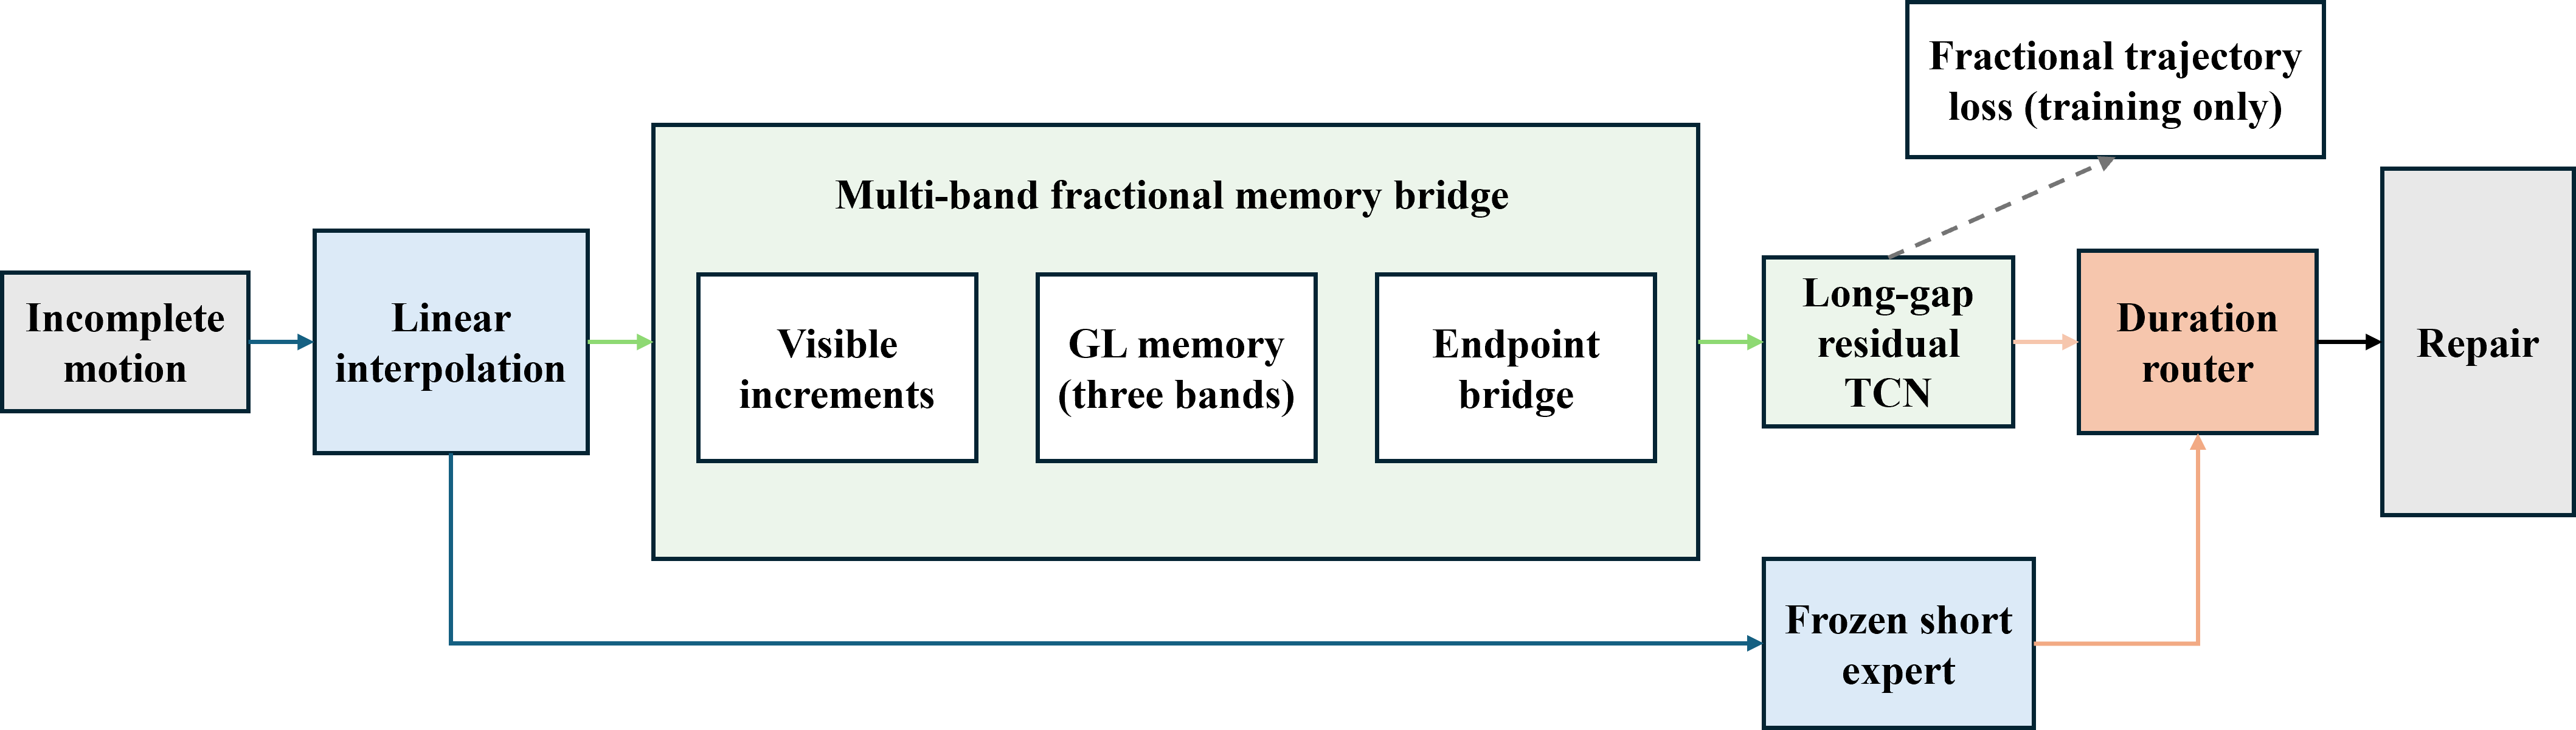
\includegraphics[width=\fulllength]{figures/figure1_fractional_method_manual.png}
\end{adjustwidth}
\caption{Architecture of the proposed endpoint-constrained multi-band fractional memory system. A linear estimate is refined by duration-specialized short- and long-gap experts. The long-gap expert combines visible-motion increments, three GL fractional-memory bands, endpoint-constrained integration, and a residual TCN. Missing-run duration determines expert weighting, and observed coordinates are restored exactly in the final output. The fractional trajectory loss is used only during training.\label{fig:method}}
\end{figure}

\subsection{Visible Motion Increments}

The input to the memory operator is not the interpolated position itself but a masked motion increment. Flatten joint and coordinate indices into channel $c$. Define

\begin{linenomath}
\begin{align}
d_{t,c}&=X_{\mathrm{lin},t,c}-X_{\mathrm{lin},t-1,c},\\
\nu_{t,c}&=M_{t,c}M_{t-1,c},
\label{eq:visible_increment}
\end{align}
\end{linenomath}

with $d_{0,c}=0$ and $\nu_{0,c}=0$. The memory convolution is normalized by $\nu$; therefore, $d_{t,c}$ contributes only when both frames that define it are observed. Altering any hidden ground-truth coordinate while keeping the observed input fixed cannot change the memory features. This property was verified by an automated hidden-target mutation test.

\subsection{Multi-Band GL Fractional Memory}

For fractional-integral order $\beta\in(0,1)$ and truncation length $K$, the nonnegative GL coefficients are generated by

\begin{linenomath}
\begin{align}
\widetilde{w}^{(\beta)}_0&=1,\\
\widetilde{w}^{(\beta)}_k&=\widetilde{w}^{(\beta)}_{k-1}\frac{\beta+k-1}{k},\quad k=1,\ldots,K-1,\\
w^{(\beta)}_k&=\frac{\widetilde{w}^{(\beta)}_k}{\sum_{q=0}^{K-1}\widetilde{w}^{(\beta)}_q}.
\label{eq:gl_integral}
\end{align}
\end{linenomath}

Asymptotically, $w_k^{(\beta)}$ follows a power law proportional to $k^{\beta-1}$, producing graded long memory. We use $K=97$ and three bounded order bands: $[0.10,0.35]$, $[0.35,0.65]$, and $[0.65,0.90]$. The order is shared across the $x$, $y$, and $z$ coordinates of each joint. The confirmatory model allowed orders to move within their bands; a later ablation tests whether that adaptation matters.

For each band $b$, visible past and future increments are combined with one mask-normalized bidirectional operator:

\begin{linenomath}
\begin{equation}
h^{(b)}_{t,c}=
\frac{\sum_{k=0}^{K-1}w^{(\beta_b)}_{k,c}
\left(\nu_{t-k,c}d_{t-k,c}+\nu_{t+k,c}d_{t+k,c}\right)}
{\sum_{k=0}^{K-1}w^{(\beta_b)}_{k,c}
\left(\nu_{t-k,c}+\nu_{t+k,c}\right)+\epsilon}-d_{t,c},
\label{eq:bidirectional_context}
\end{equation}
\end{linenomath}

where out-of-range indices contribute zero. Three band features are mixed by channel-wise softmax weights $\pi_{c,b}$. A learned $1\times1$ channel projection $\mathbf{W}$ and sigmoid gate $a_c$ produce residual increments

\begin{linenomath}
\begin{equation}
r_{t,c}=\sigma(a_c)\left[\mathbf{W}\left(\sum_{b=1}^{3}\pi_{c,b}h^{(b)}_{t,c}\right)\right]_t.
\label{eq:residual_increment}
\end{equation}
\end{linenomath}

The projection is initialized to zero, so fine-tuning begins from the original long expert rather than from a perturbed trajectory.

\subsection{Endpoint-Constrained Residual Bridge}

Consider a bounded missing run $t=a+1,\ldots,b-1$ with observed endpoints $a$ and $b$. Directly accumulating $r_t$ would generally displace the trajectory at frame $b$. We instead define

\begin{linenomath}
\begin{equation}
c_{t,c}=\sum_{u=a+1}^{t}r_{u,c}-\frac{t-a}{b-a}\sum_{u=a+1}^{b}r_{u,c},
\quad a<t<b.
\label{eq:endpoint_bridge}
\end{equation}
\end{linenomath}

The correction is set to zero outside missing entries. Equation~(\ref{eq:endpoint_bridge}) is a discrete bridge: evaluating its cumulative form at either endpoint gives zero. The memory-adjusted position supplied to the long TCN is

\begin{linenomath}
\begin{equation}
\mathbf{Z}=\mathbf{X}_{\mathrm{lin}}+\mathbf{C}.
\label{eq:adjusted_signal}
\end{equation}
\end{linenomath}

The TCN receives $\mathbf{Z}$ concatenated with the visibility mask and predicts a residual relative to $\mathbf{X}_{\mathrm{lin}}$. Equation~(\ref{eq:router_output}) then restores every observed coordinate exactly. Leading or trailing gaps without two observed boundaries do not receive the endpoint bridge; they retain the interpolation initialization and TCN correction.

\subsection{Finite-Window Control}

The finite control replaces the three GL kernels with uniform averages over 9, 33, and 97 frames. It retains the visible-increment rule, bidirectional mask normalization, three-band mixing, channel projection, sigmoid gate, endpoint bridge, long TCN, and duration router. The fractional and finite long experts each contain 1,511,739 nominal trainable parameters, and each complete two-expert system contains 3,020,622 parameters. In the finite implementation, 51 order logits are retained to match tensor count but are inactive because uniform kernels have no order. Discounting these logits changes active capacity by only 0.0034\% of the long expert, preserving a parameter-matched comparison.

\subsection{Training Objective and Optimization}

The long expert is initialized from the corresponding original DanceRouter checkpoint for each seed. Training uses a uniform curriculum over 32- and 48-frame full-body gaps, 48- and 72-frame one-limb gaps, and mixed missingness. Position loss is mean Euclidean error over missing joints. Velocity loss covers transitions touching a missing entry, and bone loss is the smooth-$L_1$ relative bone-length discrepancy:

\begin{linenomath}
\begin{equation}
\mathcal{L}_{\mathrm{base}}=\mathcal{L}_{\mathrm{pos}}+0.15\mathcal{L}_{\mathrm{vel}}+0.10\mathcal{L}_{\mathrm{bone}}.
\label{eq:base_loss}
\end{equation}
\end{linenomath}

The confirmatory fractional model also used a short-window GL trajectory loss following Guo et al. \cite{guo2026fotsr}. For derivative order $\alpha$, its coefficients satisfy

\begin{linenomath}
\begin{align}
q^{(\alpha)}_0&=1,\\
q^{(\alpha)}_k&=-q^{(\alpha)}_{k-1}\frac{\alpha-k+1}{k}.
\label{eq:gl_difference}
\end{align}
\end{linenomath}

Let $D^{\alpha}_{K_f}$ denote the average of left- and right-sided convolutions with the first $K_f$ coefficients. The training-only trajectory term is

\begin{linenomath}
\begin{equation}
\mathcal{L}_{\mathrm{frac}}=
\frac{\sum_{t,j}(1-M_{t,j})
\left\|D^{\alpha}_{K_f}\widehat{\mathbf{X}}_{t,j}
-D^{\alpha}_{K_f}\mathbf{X}_{t,j}\right\|_2}
{\sum_{t,j}(1-M_{t,j})}.
\label{eq:fractional_loss}
\end{equation}
\end{linenomath}

We set $\alpha=0.5$, $K_f=5$, and optimize $\mathcal{L}_{\mathrm{base}}+0.1\mathcal{L}_{\mathrm{frac}}$. This five-frame derivative penalty is distinct from the 97-frame fractional-integral memory in Equations~(\ref{eq:gl_integral})--(\ref{eq:residual_increment}). Because the finite bridge used $\mathcal{L}_{\mathrm{base}}$, we additionally trained the fractional bridge with $\mathcal{L}_{\mathrm{base}}$ alone for all three seeds. This loss-matched mechanism control used the same initialization policy, masks, optimization schedule, and test protocol. It was specified after the confirmatory analysis and is therefore reported as post-confirmatory rather than as a second independent confirmation.

AdamW \cite{loshchilov2019adamw} uses backbone learning rate $10^{-4}$, memory-adapter learning rate $10^{-3}$, weight decay $10^{-4}$, batch size 16, gradient clipping at 1, and mixed precision. Fine-tuning lasts at most eight epochs. Each epoch samples two 128-frame windows per training sequence. Validation uses three fixed windows per sequence and selects the lowest predefined relative primary score.

\subsection{Dataset, Preprocessing, and Grouped Split}

We use all 1,408 AIST++ sequences and their released 3D COCO-format keypoints \cite{li2021aist}. The 1,123,873 aligned frames are retained at the native 60 Hz. Each pose is centered at the pelvis, and each sequence is divided by its median torso length. Position errors are therefore reported in torso-normalized units, not millimeters.

The split unit is the combination of dance genre and choreography identifier. Every recording of a held-out choreography remains outside training. Split seed 20260829 yields 1,002 training, 185 validation, and 221 test sequences. Test windows have length 128, stride 128, and include the final valid window, producing 1,419 windows. Training seeds are 20260829, 20260830, and 20260831. Test masks use a fixed independent seed, 20270829, shared across methods and training seeds.

\begin{table}[H]
\caption{Dataset and experimental protocol.\label{tab:protocol}}
\begin{tabularx}{\textwidth}{lX}
\toprule
\textbf{Item} & \textbf{Setting}\\
\midrule
Dataset & AIST++ released 3D COCO keypoints; 1,408 sequences; 1,123,873 frames\\
Representation & 17 joints; pelvis centered; sequence torso normalized; native 60 Hz\\
Windowing & 128 frames (2.133 s); no temporal resampling\\
Group split & Genre + choreography; 1,002/185/221 train/validation/test sequences\\
Training seeds & 20260829, 20260830, and 20260831\\
Confirmatory endpoint & Missing-entry MPJPE for one-limb, 72-frame occlusion\\
Confirmatory masks & Fixed seed 20270829; identical across methods and seeds\\
Test aggregation & Seed-averaged prediction errors at sequence level\\
Inference statistics & 10,000 paired bootstrap resamples of 221 held-out sequences\\
Exploratory sweep & Limb gaps of 24, 36, 48, 60, 72, 84, and 96 frames; 3 mask repeats\\
\bottomrule
\end{tabularx}
\end{table}

\subsection{Development and Confirmatory Protocol}

The initial development gate required the fractional bridge to beat the finite bridge by at least 0.2\% on an aggregate of 48-frame limb, 72-frame limb, and mixed masks, with no screened condition regressing by more than 1.5\% against the original router. Across three seeds, the aggregate fractional advantage was 0.0756\% $\pm$ 0.0659\% and did not meet the gate. The grouped test set was not accessed during this decision.

The same development runs showed consistent 72-frame limb gains of 0.2815\%, 0.2808\%, and 0.2983\%. Before test access, we fixed a focused hypothesis with four requirements: positive gain in every seed, at least 0.2\% gain after sequence-level seed averaging, a 10,000-resample paired bootstrap interval excluding zero, and no partial-body secondary regression above 1.5\%. No model, checkpoint, mask, route threshold, or optimization setting changed after that protocol was written. Figure~\ref{fig:protocol} summarizes the separation between model development, held-out evaluation, and the subsequent exploratory analysis.

\begin{figure}[H]
\begin{adjustwidth}{-\extralength}{0cm}
\centering
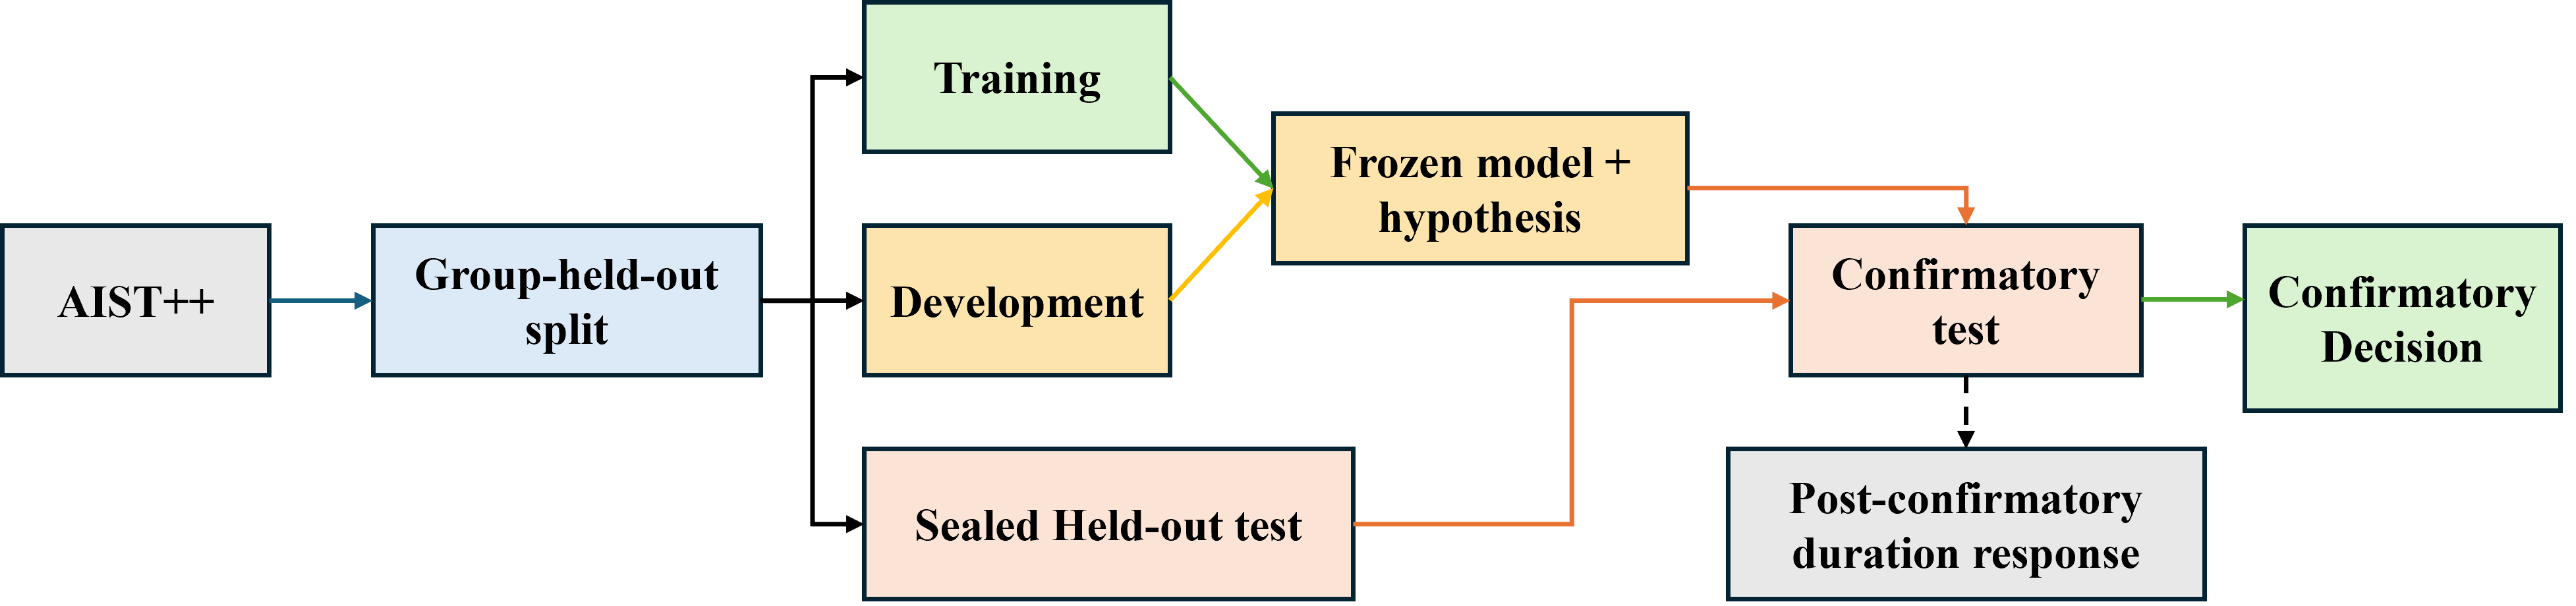
\includegraphics[width=\fulllength]{figures/figure2_evaluation_protocol_manual.png}
\end{adjustwidth}
\caption{Experimental protocol separating model development from held-out evaluation. Training and development data were used to select the model and the focused 72-frame limb-occlusion hypothesis. The grouped test split was evaluated only after the model, hypothesis, and decision rules had been fixed. The duration-response analysis was conducted after the primary evaluation and is reported as exploratory.\label{fig:protocol}}
\end{figure}

\subsection{Metrics, Statistics, and Efficiency}

The primary metric is mean per-joint position error (MPJPE) over missing entries. Secondary metrics are Euclidean velocity error on affected transitions and relative bone-length error. For each held-out sequence, errors are first averaged across its windows and the three training seeds. Method differences are then paired by sequence. We report relative gain, percentile 95\% confidence intervals from 10,000 bootstrap resamples \cite{efron1994bootstrap}, sequence win fraction, and paired Cohen's $d_z$. A positive gain means the second method has lower error.

The duration sweep was specified after the focused test and is exploratory. It evaluates seven limb-gap lengths with three fixed mask repeats per training seed, giving nine paired replicates per sequence and method. Spearman correlation describes the association between gap duration and fractional gain; it is not treated as an independent confirmatory test.

Latency is measured on an NVIDIA RTX 3090 after 100 warm-up passes and 500 timed repetitions. CUDA synchronization brackets every measurement. Batch sizes 1 and 32 are reported, together with peak allocated GPU memory. All automatic tests verify checkpoint compatibility, equal nominal parameter count, exact observation preservation, finite gradients, and invariance to mutation of hidden targets.

\subsection{Use of Generative Artificial Intelligence}

OpenAI Codex (GPT-5, accessed 3 September 2026) assisted with language editing, manuscript organization, technical scripting, and figure-layout planning. The tool was not used to generate experimental observations. All experiments ran in the authors' computing environment, and the authors verified the code, numerical results, citations, figures, and final text.

\section{Results}

\subsection{Broad Development Gate and Focused Confirmation}

The broad development claim was not supported. Fractional memory improved the 72-frame localized limb condition in every seed, but it was inconsistent for 48-frame limb and mixed masks and worse for 32- and 48-frame full-body gaps. Accordingly, only the focused 72-frame limb hypothesis was carried into confirmatory interpretation.

On the held-out test set, all three seed-specific fractional-versus-finite MPJPE gains were positive and met the 0.2\% threshold: 0.341\%, 0.237\%, and 0.203\%. After seed averaging at the sequence level, the relative gain was 0.279\% with 95\% CI [0.167, 0.387]\%, sequence win fraction 62.4\%, and paired $d_z=0.312$. All four pre-specified confirmation requirements were met.

Table~\ref{tab:main_results} separates the endpoint-bridge contribution from the fractional-kernel contribution. The finite bridge reduced MPJPE by 5.293\% relative to the original router, and the complete fractional system reduced it by 5.556\%. The bridge formulation and renewed long-expert training provide the dominant system-level improvement; replacing finite windows with power-law kernels supplies an additional 0.279\% pairwise reduction for the targeted long-limb condition.

\begin{table}[H]
\caption{Held-out 72-frame limb-occlusion results averaged over three training seeds. Error entries are mean $\pm$ sample standard deviation across seeds. Latency is the strict batch-1 median from a separate 500-repetition benchmark. Lower error is better.\label{tab:main_results}}
\begin{adjustwidth}{-\extralength}{0cm}
\scriptsize
\begin{tabular}{lrrrrr}
\toprule
\textbf{Method} & \textbf{MPJPE} & \textbf{Velocity error} & \textbf{Bone error} & \textbf{Parameters} & \textbf{Latency (ms)}\\
\midrule
Original DanceRouter & $0.259212\pm0.001188$ & $0.029467\pm0.000206$ & $0.080294\pm0.001345$ & 3,017,766 & 4.208\\
Finite-window bridge & $0.245765\pm0.000141$ & $0.029176\pm0.000145$ & $0.077551\pm0.000558$ & 3,020,622 & 6.297\\
Fractional bridge & $\mathbf{0.245124\pm0.000092}$ & $\mathbf{0.029160\pm0.000169}$ & $\mathbf{0.076934\pm0.000466}$ & 3,020,622 & 14.158\\
\bottomrule
\end{tabular}
\end{adjustwidth}
\end{table}

\begin{table}[H]
\caption{Paired sequence-bootstrap comparisons for the confirmatory 72-frame limb condition. Gain is positive when the second method has lower MPJPE.\label{tab:bootstrap}}
\begin{tabularx}{\textwidth}{Xrrrr}
\toprule
\textbf{Comparison} & \textbf{Gain (\%)} & \textbf{95\% CI (\%)} & \textbf{Wins (\%)} & $\mathbf{d_z}$\\
\midrule
Original $\rightarrow$ finite bridge & 5.293 & [4.757, 5.883] & 93.2 & 1.097\\
Original $\rightarrow$ fractional bridge & 5.556 & [5.019, 6.127] & 93.7 & 1.106\\
Finite $\rightarrow$ fractional bridge & 0.279 & [0.167, 0.387] & 62.4 & 0.312\\
\bottomrule
\end{tabularx}
\end{table}

\begin{figure}[H]
\begin{adjustwidth}{-\extralength}{0cm}
\centering
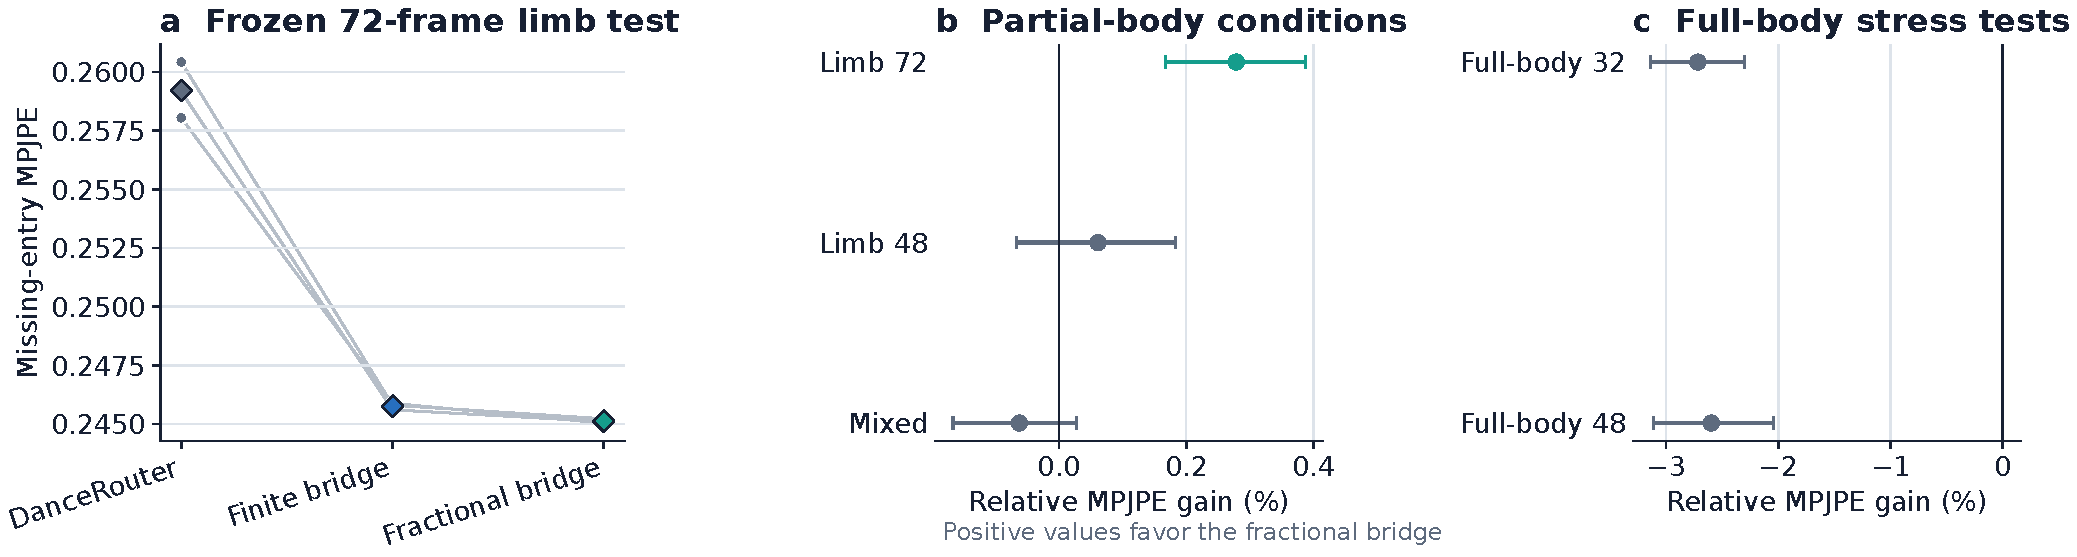
\includegraphics[width=\fulllength]{figures/figure3_confirmatory_results.pdf}
\end{adjustwidth}
\caption{Confirmatory result and scope boundary. In panel (a), circles are seed-specific errors and diamonds are three-seed means. Panels (b,c) show paired sequence-bootstrap estimates and 95\% confidence intervals. The fractional bridge reduces MPJPE for the focused 72-frame limb condition; secondary partial-body intervals include zero, and uniform full-body temporal holes favor finite memory.\label{fig:confirmatory}}
\end{figure}

\subsection{Loss-Matched Memory Control}

The confirmatory fractional system differed from the finite bridge in both its inference kernel and its training-only fractional trajectory loss. We therefore repeated the three-seed fractional training with $\mathcal{L}_{\mathrm{frac}}$ removed. Under the same 72-frame limb masks, seed-specific MPJPE gains over the finite bridge were 0.349\%, 0.242\%, and 0.217\%. After sequence-level seed averaging, the loss-matched gain was 0.293\% (95\% CI [0.184, 0.400]\%), the sequence win fraction was 62.9\%, and paired $d_z=0.332$. The mean MPJPE was $0.245102\pm0.000098$, compared with $0.245765\pm0.000141$ for the finite bridge.

The loss-matched positional gain is comparable to the 0.279\% complete-system gain, showing that the short-window fractional trajectory penalty is not required for the observed MPJPE improvement. Bone error also remained lower than with finite memory (0.076987 versus 0.077551), whereas velocity error was marginally higher (0.029197 versus 0.029176). The persistence of the position and bone effects supports an inference-side contribution from fractional memory; the change in the velocity result is consistent with the trajectory loss contributing to that secondary metric. This control was conducted after the primary test and is treated as a mechanism analysis.

\begin{table}[H]
\caption{Post-confirmatory loss-matched control for the 72-frame limb condition. Both methods use $\mathcal{L}_{\mathrm{base}}$ and have the same nominal parameter count. Gain is positive when fractional memory has lower MPJPE.\label{tab:loss_matched}}
\begin{tabularx}{\textwidth}{Xrrr}
\toprule
\textbf{Comparison} & \textbf{Seed gains (\%)} & \textbf{Aggregate gain (\%)} & \textbf{95\% CI (\%)}\\
\midrule
Finite bridge $\rightarrow$ fractional bridge & 0.349 / 0.242 / 0.217 & 0.293 & [0.184, 0.400]\\
\bottomrule
\end{tabularx}
\end{table}

\subsection{Secondary Conditions Define the Scope}

Table~\ref{tab:scope} defines the observed scope. The 48-frame limb and mixed-mask intervals include zero, while uniform 32- and 48-frame full-body holes increase fractional-bridge MPJPE by approximately 2.6--2.7\% relative to the finite bridge. Localized limb outages retain visible torso and contralateral motion for bidirectional aggregation, whereas full-body holes remove this contemporaneous skeletal context. One possible explanation is that power-law increment aggregation over-smooths or misaligns the transition when all joints are absent simultaneously.

\begin{table}[H]
\caption{Fractional-versus-finite MPJPE comparisons across pre-specified secondary conditions. Positive gain favors fractional memory.\label{tab:scope}}
\begin{tabularx}{\textwidth}{lrrr>{\raggedright\arraybackslash}X}
\toprule
\textbf{Condition} & \textbf{Gain (\%)} & \textbf{95\% CI (\%)} & \textbf{Wins (\%)} & \textbf{Interpretation}\\
\midrule
One-limb gap, 72 frames & 0.279 & [0.167, 0.387] & 62.4 & Fractional better; confirmatory\\
One-limb gap, 48 frames & 0.061 & [-0.066, 0.184] & 53.4 & No resolved difference\\
Mixed missingness & -0.062 & [-0.166, 0.027] & 48.0 & No resolved difference\\
Full-body gap, 32 frames & -2.718 & [-3.137, -2.304] & 10.4 & Finite better\\
Full-body gap, 48 frames & -2.597 & [-3.113, -2.041] & 10.9 & Finite better\\
\bottomrule
\end{tabularx}
\end{table}

\subsection{Exploratory Duration Response}

The post-confirmatory sweep clarifies when the fractional profile begins to help (Figure~\ref{fig:duration}). MPJPE differences are unresolved at 24, 36, and 48 frames. The fractional gain becomes significant at 60 frames (0.185\%, 95\% CI [0.096, 0.276]\%), rises to 0.242\% at 72 frames and 0.284\% at 84 frames, and remains significant at 96 frames (0.271\%). The association between duration and MPJPE gain is strong (Spearman $\rho=0.964$), although it is not strictly monotonic because the 96-frame point is slightly below the 84-frame point.

The relative change is larger for bone-length consistency than for position. Bone-length-error gains are significant from 48 frames onward and reach 0.749\%, 0.971\%, 1.238\%, and 1.175\% at 60, 72, 84, and 96 frames, respectively. Velocity gains become significant at 60 frames and remain between 0.083\% and 0.118\% through 96 frames. The larger bone-length effect, together with the positive velocity effect, is consistent with improved kinematic continuity rather than a large change in pointwise position error.

\begin{figure}[H]
\begin{adjustwidth}{-\extralength}{0cm}
\centering
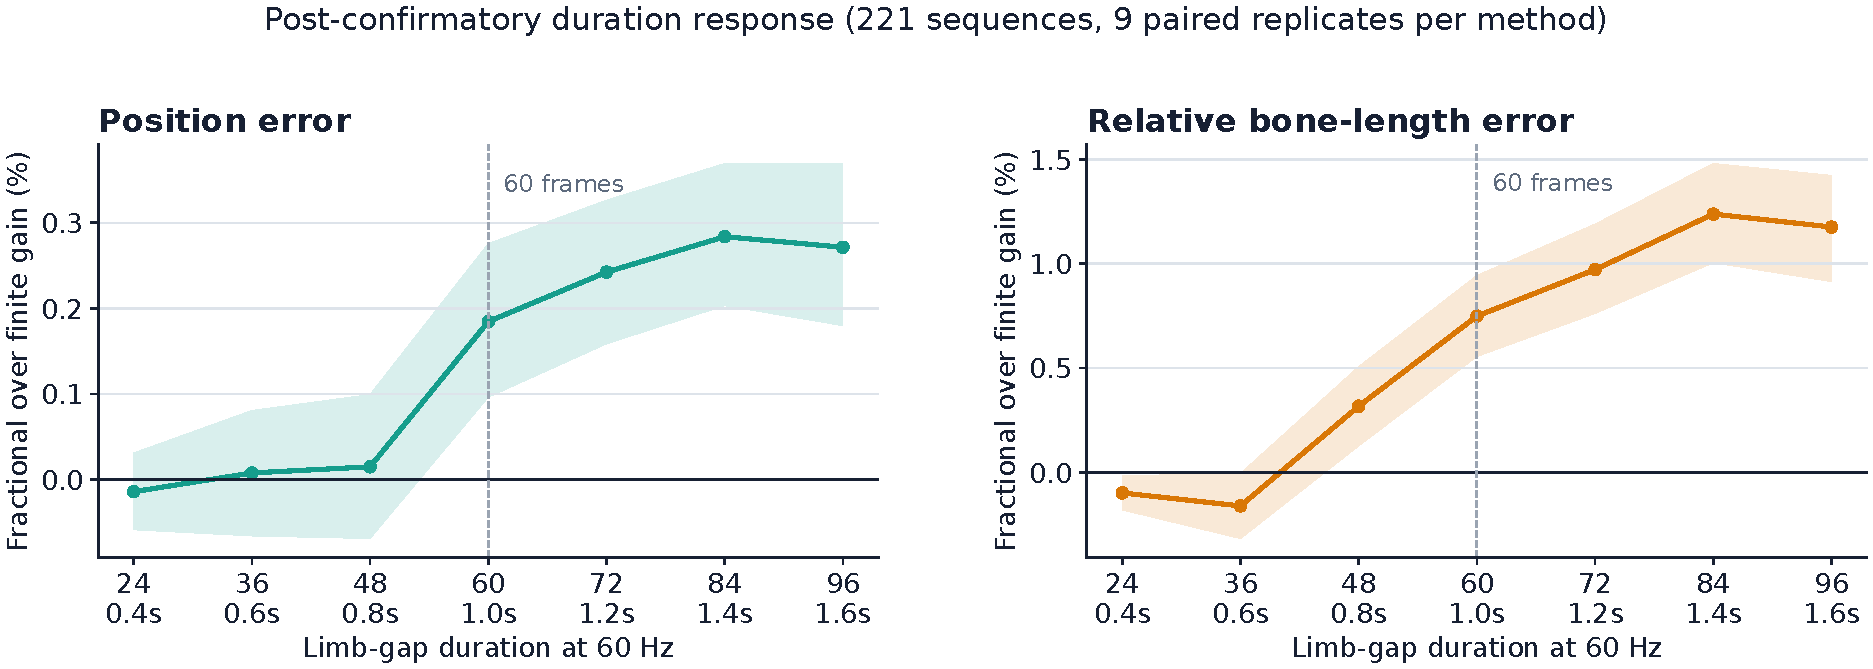
\includegraphics[width=\fulllength]{figures/figure4_duration_response.pdf}
\end{adjustwidth}
\caption{Post-confirmatory duration response for localized limb gaps. Each point aggregates 221 sequences, three training seeds, and three fixed mask repeats; shaded bands are paired 95\% bootstrap intervals. The analysis is exploratory because its duration grid was specified after the focused test.\label{fig:duration}}
\end{figure}

\subsection{Memory Parameters and Order Ablation}

Across seeds and joints, the learned mean orders were 0.199, 0.474, and 0.754 for the three bands. Mean channel mixture weights were 0.434, 0.287, and 0.279, and the mean sigmoid gate was 0.156. These values indicate that the long expert uses the memory bridge as a restrained correction and assigns the largest average mass to the fastest-decaying band while retaining substantial contributions from the two longer-memory bands.

On the development validation split, fixed band centers $(0.225,0.500,0.775)$ improved MPJPE by 0.0239\% relative to learned joint-specific orders. Collapsing the orders to their joint mean or permuting them across joints also changed MPJPE by less than 0.01\%. These results provide no evidence that joint-specific order learning is necessary in this setting and support fixing the three band centers in a simpler implementation. A single-band control would be required to determine whether mixing multiple fractional profiles is itself beneficial.

\begin{table}[H]
\caption{Post-confirmatory order ablation on the development validation split under 72-frame limb occlusion. Negative relative change denotes lower MPJPE than the learned-order model.\label{tab:order_ablation}}
\begin{tabularx}{\textwidth}{Xrr}
\toprule
\textbf{Order configuration} & \textbf{Mean MPJPE} & \textbf{Change vs. learned (\%)}\\
\midrule
Learned joint-specific orders & 0.237834 & 0.0000\\
Fixed band centers & \textbf{0.237777} & -0.0239\\
Joint-mean orders & 0.237818 & -0.0069\\
Joint-permuted orders & 0.237814 & -0.0084\\
\bottomrule
\end{tabularx}
\end{table}

\begin{figure}[H]
\begin{adjustwidth}{-\extralength}{0cm}
\centering
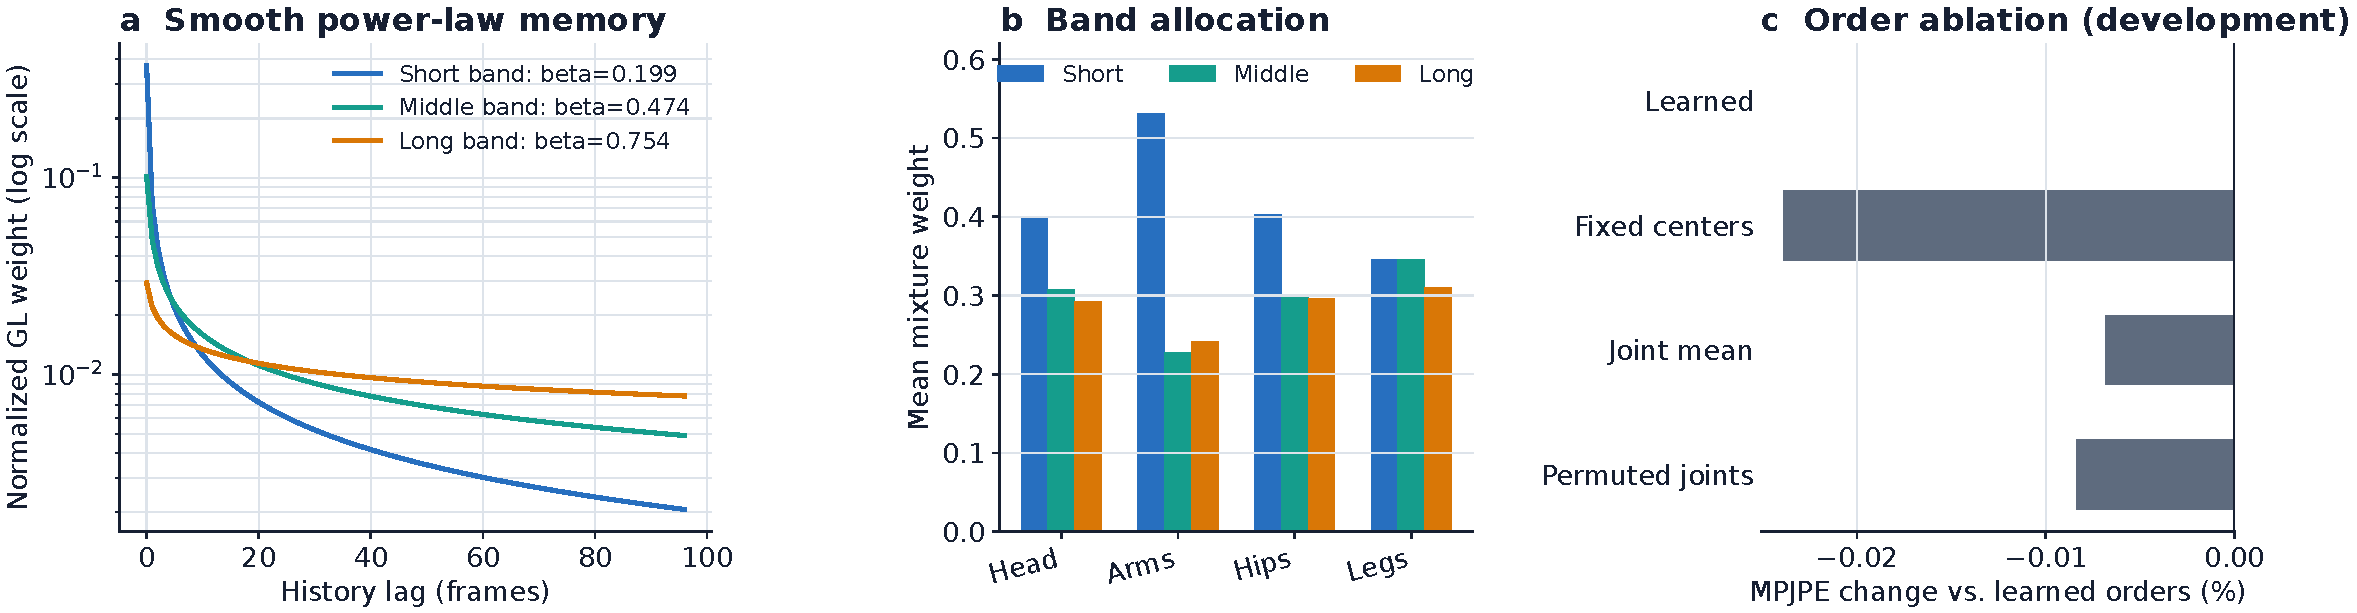
\includegraphics[width=\fulllength]{figures/figure5_memory_analysis.pdf}
\end{adjustwidth}
\caption{Fractional memory analysis. The three GL bands produce distinct power-law lag profiles and receive non-zero mixture weights across body regions. Fixed, averaged, and permuted orders match or slightly improve on learned joint-specific orders in the development ablation.\label{fig:memory}}
\end{figure}

\subsection{Efficiency and Verification}

The fractional bridge is computationally heavier than its finite counterpart. At batch size 1, median latency was 14.158 ms for the fractional system, 6.297 ms for the finite system, and 4.208 ms for the original router. The fractional 95th percentile was 15.403 ms. At batch size 32, median latency per window was 0.440, 0.195, and 0.130 ms, respectively. Peak allocated memory was 43.43 MiB for both bridge systems at batch size 32. A 128-frame window represents 2.133 s of motion, and the 14.158 ms fractional inference time supports buffered processing. Bidirectional context makes the method noncausal.

\begin{figure}[H]
\begin{adjustwidth}{-\extralength}{0cm}
\centering
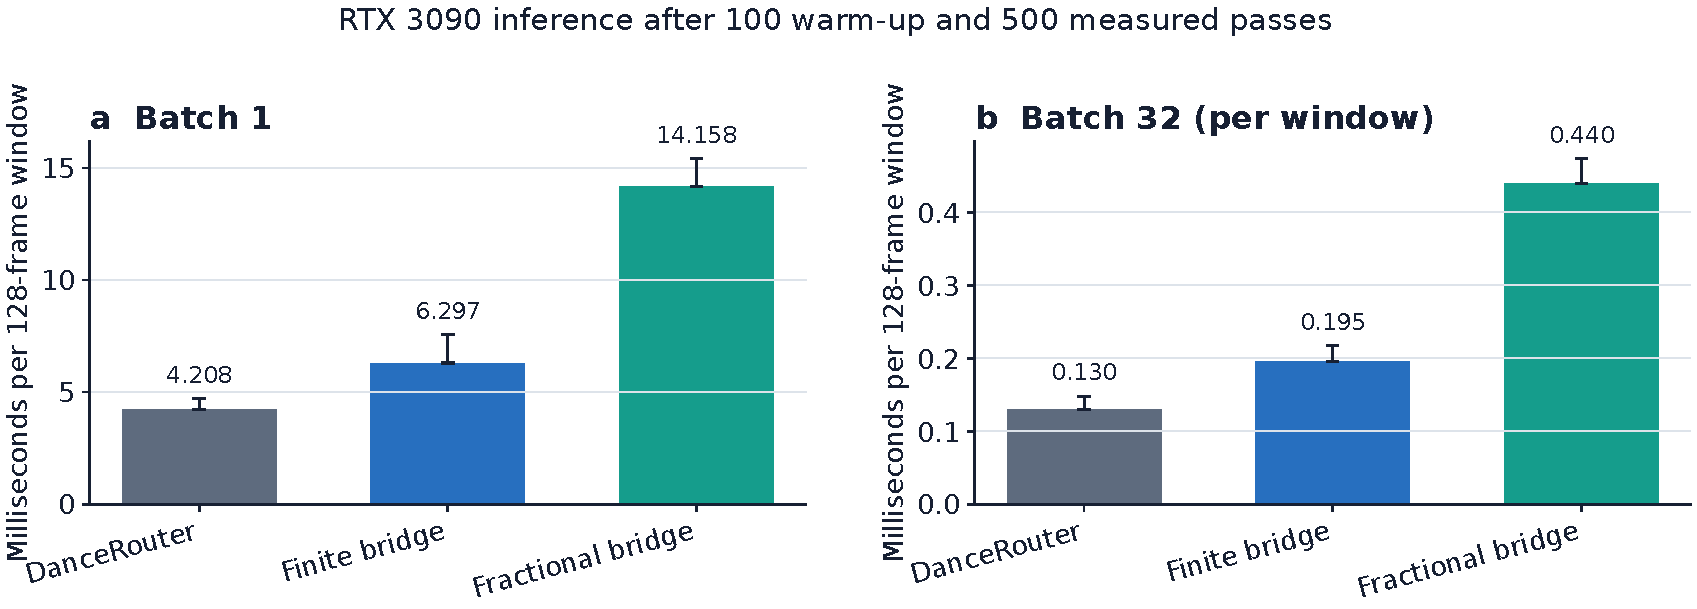
\includegraphics[width=\fulllength]{figures/figure6_efficiency.pdf}
\end{adjustwidth}
\caption{Inference timing on an RTX 3090 after 100 warm-up and 500 measured passes. Bars show median milliseconds per 128-frame window and upper whiskers show the 95th percentile. Fractional inference takes 14.158 ms per window at batch size 1, compared with 6.297 ms for the finite bridge.\label{fig:efficiency}}
\end{figure}

All verification tests passed. Fractional and finite models preserve observed coordinates exactly after projection; mutating hidden targets does not affect predictions; finite and fractional bridge checkpoints load into the intended architectures; all tested gradients are finite; and the endpoint correction is numerically zero at observed boundaries.

\section{Discussion}

\subsection{What the Fractional Operator Adds}

The endpoint bridge provides the dominant system-level improvement over the original duration router: the finite bridge reduces MPJPE by 5.293\%, and the fractional system reduces it by 5.556\%. In the complete-system comparison, replacing finite-window averages with power-law GL profiles and adding the trajectory term yields a further 0.279\% MPJPE reduction for a 1.2 s localized limb outage. The loss-matched control retains a 0.293\% reduction, showing that the positional improvement persists without the extra trajectory loss. Both intervals exclude zero, all training seeds agree, and approximately 63\% of held-out sequences favor fractional memory. Thus, the fractional kernel acts as a consistent incremental refinement in the tested condition, while the endpoint bridge remains the main source of the system-level gain.

The duration response identifies where graded temporal history becomes useful in this dataset. No MPJPE advantage is resolved for 24--48-frame gaps, while the difference favors fractional memory from 60 to 96 frames. One interpretation is that narrow finite windows cannot span the longer outage, whereas wide uniform windows give the same weight to recent and distant increments. The power-law profiles retain the full 97-frame context while attenuating older increments. The response is not strictly monotonic because the 96-frame point lies slightly below the 84-frame point.

The endpoint constraint is central to the application. Fractional accumulation without detrending can shift the trajectory where a joint reappears. Equation~(\ref{eq:endpoint_bridge}) removes this displacement analytically and separates memory shape from boundary consistency. The visible-increment mask is equally important: applying a fractional operator directly to interpolated hidden points would allow the initialization to be repeatedly recycled as if it were measured evidence.

\subsection{Relation to Existing Fractional Human-Motion Methods}

Pose3DM \cite{wang2025pose3dm} and FOTSR \cite{guo2026fotsr} demonstrate that fractional regularization can improve pose stability and motion prediction. Our findings complement rather than supersede them. We use a fractional integral to construct inference features from incomplete observations, not only to penalize a complete predicted trajectory during training. The endpoint bridge also addresses an interpolation constraint absent from future prediction.

Fixed band centers match or slightly outperform learned joint-specific orders in the post-confirmatory ablation. The tested model therefore does not benefit from joint-specific order learning. A simpler implementation can fix the fractional bands and learn only their mixture and channel projection. This ablation concerns order adaptation; it does not establish that three bands are better than one.

\subsection{Implications for Dance Technology}

Dance motion contains repeated distal-limb occlusions during turns, arm crossings, level changes, and floorwork. For offline coaching or archival processing, a duration-aware implementation could reserve the fractional bridge for prolonged localized gaps and use the faster finite path elsewhere. The 60-frame transition observed here is specific to the AIST++ experiment and should be recalibrated for other capture systems and frame rates.

The method accepts visibility or quality masks from upstream monocular or multi-view pose systems. It reconstructs entries already declared unavailable before the computation of velocity, joint angles, style descriptors, or animation controls; detection of erroneous high-confidence joints remains outside the repair task.

\subsection{Limitations}

Several limitations should be considered. First, the evaluation uses one public dance dataset with synthetically imposed gaps. It covers AIST++ motion under declared missingness rather than the failure distribution of a deployed tracker; FineDance, studio markerless capture, and downstream coaching outcomes were not evaluated. Second, torso-normalized MPJPE is not a physical-distance measure.

Third, the 72-frame hypothesis was selected after the broad development criterion failed, although the grouped test set remained unopened until the focused protocol was fixed. The duration grid and loss-matched control were specified after test access and are exploratory follow-up analyses. Fourth, the complete-system test combines the fractional bridge with a fractional trajectory loss; the loss-matched control shows that the MPJPE and bone-consistency effects persist without this loss, but it was not independently pre-specified. Fifth, the order ablation does not include a single-band fractional model, so it cannot isolate the value of multi-band mixing. Finally, the bidirectional operator is noncausal, and the observed advantage is condition specific: uniform full-body gaps favor finite memory, while localized gaps below 60 frames show no resolved position advantage.

\section{Conclusions}

This study presents an endpoint-constrained multi-band GL fractional memory bridge for long localized occlusions in 3D dance motion. Visible-only increments prevent hidden-target leakage, and the analytical bridge reconnects residual corrections exactly to observed endpoints. Under a choreography-grouped, three-seed AIST++ protocol, the fractional system reduced MPJPE by 0.279\% relative to a closely matched finite bridge for 72-frame limb gaps, with a 95\% confidence interval of 0.167--0.387\%. A post-confirmatory loss-matched control retained a 0.293\% reduction without fractional trajectory regularization, and the duration analysis found improvements for localized gaps of 60--96 frames. Bone-length consistency showed larger relative gains than MPJPE, whereas uniform full-body gaps favored finite memory. These results support duration- and geometry-aware routing: fractional memory is useful as an incremental refinement for prolonged partial-body repair, while finite modeling remains preferable for shorter or body-wide gaps.

\authorcontributions{Conceptualization, L.L. and Z.L.; methodology, Z.L.; software, Z.L.; validation, Z.L.; formal analysis, Z.L.; investigation, L.L.; resources, L.L.; data curation, Z.L.; writing---original draft preparation, L.L. and Z.L.; writing---review and editing, L.L. and Z.L.; visualization, Z.L.; supervision, Z.L.; project administration, L.L.; funding acquisition, L.L. Both authors have read and agreed to the published version of the manuscript.}

\funding{This study was supported by the Scientific Research Program Funded by the Education Department of Shaanxi Provincial Government (Program No. 25JK0277).}

\institutionalreview{Not applicable. This computational study used a previously released public motion dataset and did not recruit human or animal participants.}

\informedconsent{Not applicable.}

\dataavailability{The AIST++ data analyzed in this study are available from the official project website (\url{https://google.github.io/aistplusplus_dataset/}) under the dataset providers' terms. Raw AIST++ data, sequence-level errors, and trained checkpoints are not redistributed. The protocol definitions, aggregate results, and source code used for training, evaluation, statistical analysis, and figure generation are publicly available at \url{https://github.com/liangdagongjue-code/StreetStyle/tree/main/fractional_motion_repair}.}

\acknowledgments{The authors thank the creators of AIST++ for releasing the dataset and calibration resources. During the preparation of this manuscript, the authors used OpenAI Codex (GPT-5, accessed 3 September 2026) to assist with language editing, manuscript organization, technical scripting, and figure-layout planning. The authors reviewed and verified all outputs and take full responsibility for the content of this publication.}

\conflictsofinterest{The authors declare no conflict of interest. The funder had no role in the design of the study; in the collection, analysis, or interpretation of data; in the writing of the manuscript; or in the decision to publish the results.}

\abbreviations{Abbreviations}{
The following abbreviations are used in this manuscript:\\
\noindent
\begin{tabular}{@{}ll}
AIST++ & Multi-modal 3D dance-motion dataset\\
CI & Confidence interval\\
GL & Grunwald--Letnikov\\
MPJPE & Mean per-joint position error\\
TCN & Temporal convolutional network
\end{tabular}}

\begin{adjustwidth}{-\extralength}{0cm}
\reftitle{References}
\externalbibliography{yes}
\bibliography{fractional_dance_references}
\end{adjustwidth}

\end{document}
